\hypertarget{Sound_8h}{
\section{Sound.h File Reference}
\label{Sound_8h}\index{Sound.h@{Sound.h}}
}
{\tt \#include \char`\"{}Xml\-Reader.h\char`\"{}}\par
{\tt \#include $<$list$>$}\par
{\tt \#include \char`\"{}Types.h\char`\"{}}\par
{\tt \#include \char`\"{}Partial.h\char`\"{}}\par
{\tt \#include \char`\"{}Multi\-Track.h\char`\"{}}\par
{\tt \#include \char`\"{}Collection.h\char`\"{}}\par
{\tt \#include \char`\"{}Dynamic\-Variable.h\char`\"{}}\par
{\tt \#include \char`\"{}Spatializer.h\char`\"{}}\par
{\tt \#include \char`\"{}Reverb.h\char`\"{}}\par
{\tt \#include \char`\"{}Interpolator\-Types.h\char`\"{}}\par
{\tt \#include $<$iostream$>$}\par
{\tt \#include $<$fstream$>$}\par


Include dependency graph for Sound.h:\begin{figure}[H]
\begin{center}
\leavevmode
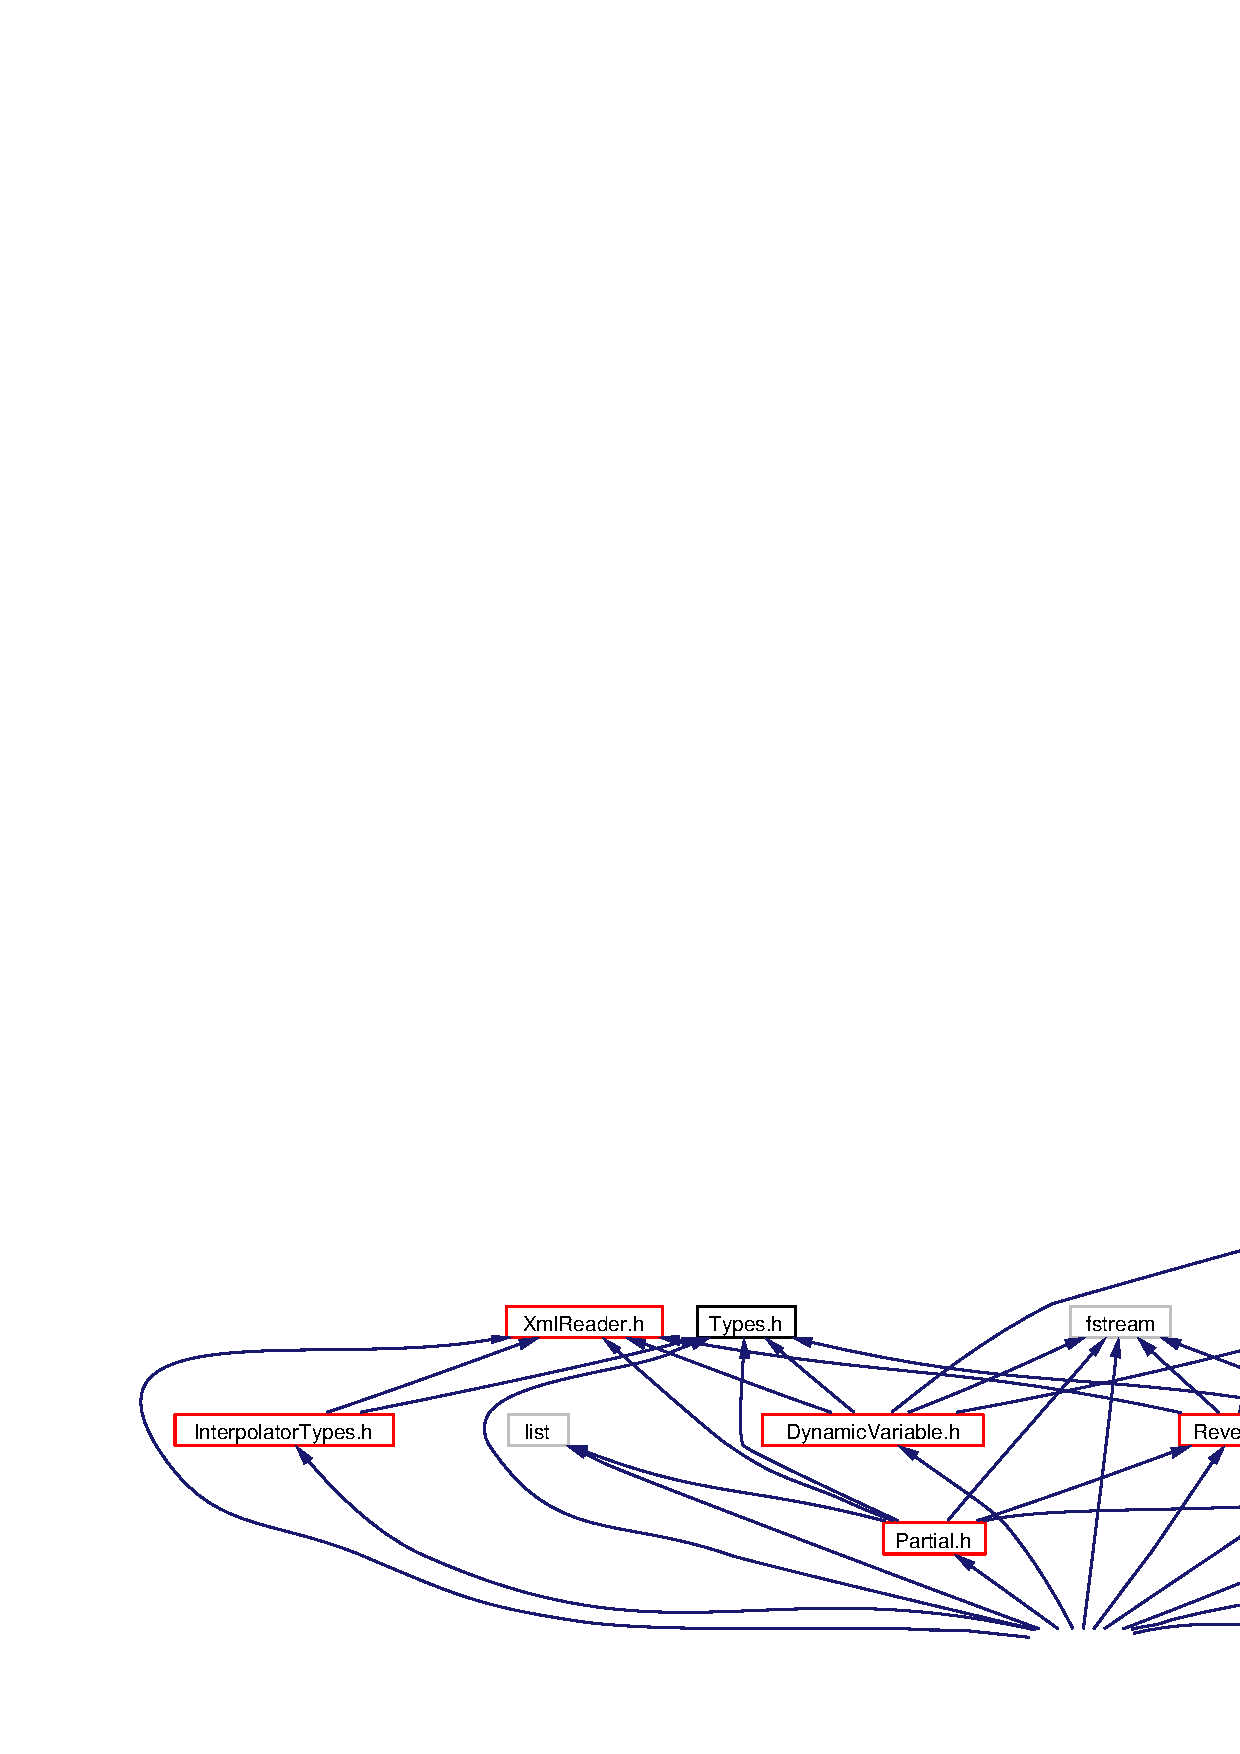
\includegraphics[width=420pt]{Sound_8h__incl}
\end{center}
\end{figure}


This graph shows which files directly or indirectly include this file:\begin{figure}[H]
\begin{center}
\leavevmode
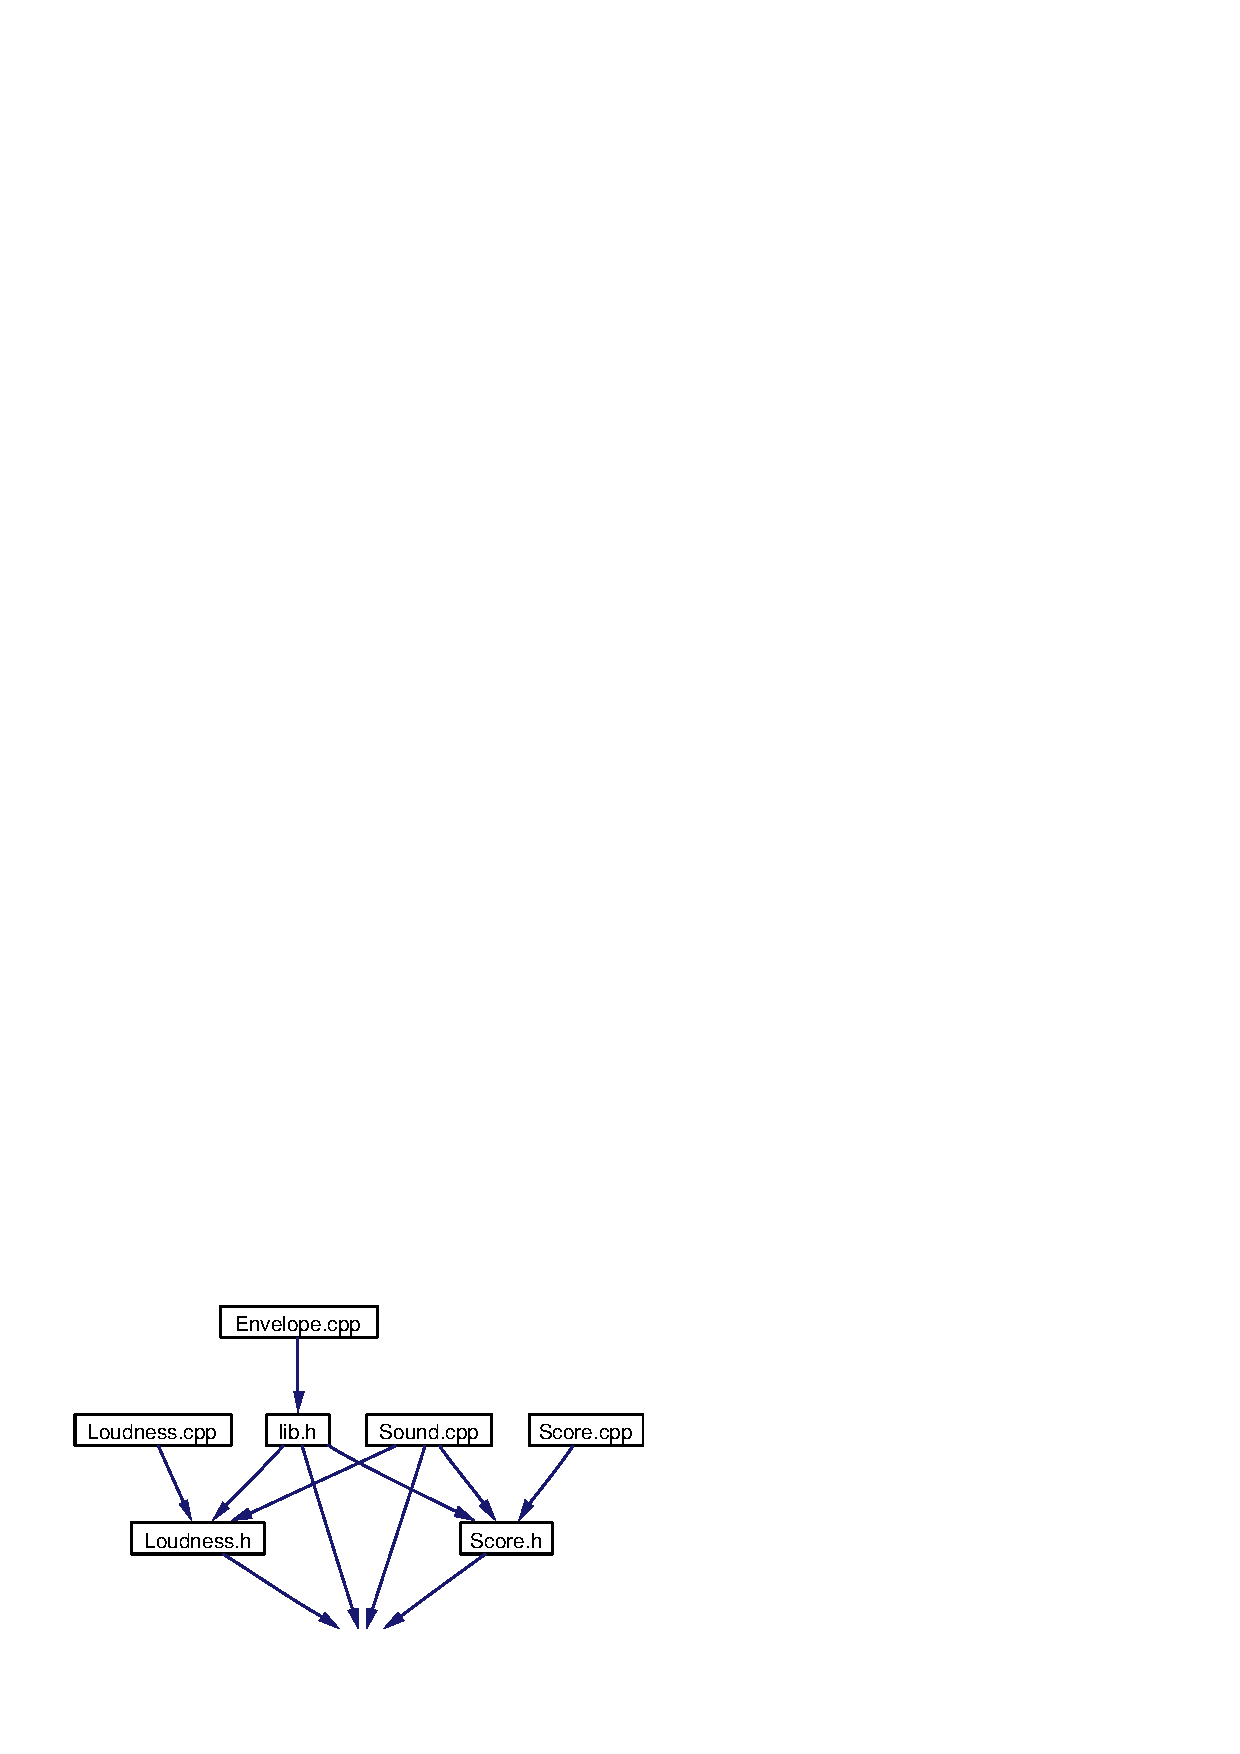
\includegraphics[width=154pt]{Sound_8h__dep__incl}
\end{center}
\end{figure}
\subsection*{Classes}
\begin{CompactItemize}
\item 
class \hyperlink{classSound}{Sound}
\end{CompactItemize}
\subsection*{Enumerations}
\begin{CompactItemize}
\item 
enum \hyperlink{Sound_8h_a8}{Sound\-Static\-Param} \{ \par
\hyperlink{Sound_8h_a8a0}{START\_\-TIME}, 
\par
\hyperlink{Sound_8h_a8a1}{DURATION}, 
\par
\hyperlink{Sound_8h_a8a2}{LOUDNESS}, 
\par
\hyperlink{Sound_8h_a8a3}{LOUDNESS\_\-RATE}, 
\par
\hyperlink{Sound_8h_a8a4}{DETUNE\_\-SPREAD}, 
\par
\hyperlink{Sound_8h_a8a5}{DETUNE\_\-DIRECTION}, 
\par
\hyperlink{Sound_8h_a8a6}{DETUNE\_\-VELOCITY}, 
\par
\hyperlink{Sound_8h_a8a7}{DETUNE\_\-FUNDAMENTAL}
 \}
\item 
enum \hyperlink{Sound_8h_a9}{Sound\-Dynamic\-Param} 
\end{CompactItemize}


\subsection{Detailed Description}
Defines a \hyperlink{classSound}{Sound} object, as well as the static and dynamic parameters that pertain to said object.

Definition in file \hyperlink{Sound_8h-source}{Sound.h}.

\subsection{Enumeration Type Documentation}
\hypertarget{Sound_8h_a9}{
\index{Sound.h@{Sound.h}!SoundDynamicParam@{SoundDynamicParam}}
\index{SoundDynamicParam@{SoundDynamicParam}!Sound.h@{Sound.h}}
\subsubsection[SoundDynamicParam]{\setlength{\rightskip}{0pt plus 5cm}enum \hyperlink{Sound_8h_a9}{Sound\-Dynamic\-Param}}}
\label{Sound_8h_a9}


Defines the Dynamic\-Parameters that can be set for a \hyperlink{classSound}{Sound} object. 

Definition at line 134 of file Sound.h.\hypertarget{Sound_8h_a8}{
\index{Sound.h@{Sound.h}!SoundStaticParam@{SoundStaticParam}}
\index{SoundStaticParam@{SoundStaticParam}!Sound.h@{Sound.h}}
\subsubsection[SoundStaticParam]{\setlength{\rightskip}{0pt plus 5cm}enum \hyperlink{Sound_8h_a8}{Sound\-Static\-Param}}}
\label{Sound_8h_a8}


\begin{Desc}
\item[Enumeration values: ]\par
\begin{description}
\index{START_TIME@{START\_\-TIME}!Sound.h@{Sound.h}}\index{Sound.h@{Sound.h}!START_TIME@{START\_\-TIME}}\item[{\em 
\hypertarget{Sound_8h_a8a0}{
START\_\-TIME}
\label{Sound_8h_a8a0}
}]\begin{itemize}
\item When placed in a \hyperlink{classScore}{Score}, the sound will start at this time. \end{itemize}
\index{DURATION@{DURATION}!Sound.h@{Sound.h}}\index{Sound.h@{Sound.h}!DURATION@{DURATION}}\item[{\em 
\hypertarget{Sound_8h_a8a1}{
DURATION}
\label{Sound_8h_a8a1}
}]\begin{itemize}
\item The sound lasts this long (in seconds) \end{itemize}
\index{LOUDNESS@{LOUDNESS}!Sound.h@{Sound.h}}\index{Sound.h@{Sound.h}!LOUDNESS@{LOUDNESS}}\item[{\em 
\hypertarget{Sound_8h_a8a2}{
LOUDNESS}
\label{Sound_8h_a8a2}
}]\begin{itemize}
\item Describes how loud the sound should be perceived at its loudest point.\item Given in Sones, the valid range is \mbox{[}0,255\mbox{]} \end{itemize}
\index{LOUDNESS_RATE@{LOUDNESS\_\-RATE}!Sound.h@{Sound.h}}\index{Sound.h@{Sound.h}!LOUDNESS_RATE@{LOUDNESS\_\-RATE}}\item[{\em 
\hypertarget{Sound_8h_a8a3}{
LOUDNESS\_\-RATE}
\label{Sound_8h_a8a3}
}]\begin{itemize}
\item \hyperlink{classLoudness}{Loudness} does not have to be calculated EVERY sample.\item This specifies how often loudness is calculated.\item the default is 10Hz. \end{itemize}
\index{DETUNE_SPREAD@{DETUNE\_\-SPREAD}!Sound.h@{Sound.h}}\index{Sound.h@{Sound.h}!DETUNE_SPREAD@{DETUNE\_\-SPREAD}}\item[{\em 
\hypertarget{Sound_8h_a8a4}{
DETUNE\_\-SPREAD}
\label{Sound_8h_a8a4}
}]\begin{itemize}
\item Detuning describes the effect of letting all partials exponentially converge from random points to their intended frequencies, or to diverge in the reverse fashion\item Detuning spread refers to the the variance in frequences at the divergent end of the sound (the beginning for convergence (tuning), the end for divergence (detuning))\item A value of 0.0 effectively disables detuning\item A value of, say, 0.3 causes the detuned frequencies to fall within the range \mbox{[}(1.0-0.3)$\ast$Freq, (1.0+0.3)$\ast$Freq\mbox{]}. In other words, the SPREAD value is a percent that corresponds to a range in which the partial will (randomly) fall at the max. detuning portion of the sound. \end{itemize}
\index{DETUNE_DIRECTION@{DETUNE\_\-DIRECTION}!Sound.h@{Sound.h}}\index{Sound.h@{Sound.h}!DETUNE_DIRECTION@{DETUNE\_\-DIRECTION}}\item[{\em 
\hypertarget{Sound_8h_a8a5}{
DETUNE\_\-DIRECTION}
\label{Sound_8h_a8a5}
}]\begin{itemize}
\item -1.0 means do detuning (divergence)\item +1.0 means do tuning (convergence) \end{itemize}
\index{DETUNE_VELOCITY@{DETUNE\_\-VELOCITY}!Sound.h@{Sound.h}}\index{Sound.h@{Sound.h}!DETUNE_VELOCITY@{DETUNE\_\-VELOCITY}}\item[{\em 
\hypertarget{Sound_8h_a8a6}{
DETUNE\_\-VELOCITY}
\label{Sound_8h_a8a6}
}]\begin{itemize}
\item Values over \mbox{[}-1.0, +1.0\mbox{]}\item For VELOCITY=0.5, the transition will be linear from start to end. For Velocity = -1.0, the transition will be nearly instantaneous and immediate (and exponentially interpolated). For velocity +1.0, the transition will be instantaneous, but will occur at the extreme end of the sound (And will be exponentially interpolated)\item If y is the amount of tuning and x is time, think of -1.0 as a vertical line on the left (at the beginning) and then a flat horizontal line. For +1.0, the horizontal line is at the beginning (on the left), and there is a sharp transition at the right end (at the end). \end{itemize}
\index{DETUNE_FUNDAMENTAL@{DETUNE\_\-FUNDAMENTAL}!Sound.h@{Sound.h}}\index{Sound.h@{Sound.h}!DETUNE_FUNDAMENTAL@{DETUNE\_\-FUNDAMENTAL}}\item[{\em 
\hypertarget{Sound_8h_a8a7}{
DETUNE\_\-FUNDAMENTAL}
\label{Sound_8h_a8a7}
}]\begin{itemize}
\item Positive values = TRUE (tune/detune the fundamental)\item Negative Values = FALSE (do not tune/detune ...) \end{itemize}
\end{description}
\end{Desc}



Definition at line 118 of file Sound.h.